\documentclass[a4paper,UTF8]{ctexart}

\usepackage{amsmath, amsthm, amssymb, amsfonts, hyperref, mathrsfs}%美国数学学会的包+?
\usepackage{geometry} %控制界面
\usepackage{bookmark}
\usepackage{fancyhdr} % header & footer
\usepackage{appendix} % 附录
\usepackage{tikz} %作图
\usepackage{graphicx} %插入图片的宏包
\usepackage{float} %设置图片浮动位置的宏包
%\usepackage{subfigure} %插入多图时用子图显示的宏包
\usepackage{listings} %引用代码
\usepackage{physics,mathtools} %物理数学工具
\usepackage{comment}
\usepackage{framed}
\usepackage{caption}
\usepackage{subcaption}
\geometry{top=2.5cm,bottom=2.5cm,left=2.5cm,right=2.5cm} % 布局要求
\pagestyle{fancy} % fancy分格
\fancyhf{} % 清除所有页眉页脚
\renewcommand\headrulewidth{0.6pt}
\renewcommand\footrulewidth{0.6pt}
% font
\setCJKmainfont{Noto Serif CJK SC}[BoldFont={Noto Serif CJK SC Bold}, ItalicFont=]
\lhead{何金铭 PB21020660$\mid$座位号:8}
\cfoot{Quantum Key Distribution 预习报告}
\rhead{\thepage}
\lfoot{2024.4.23}
\rfoot{USTC}
%\bibliographystyle{plain} % 引用样式
\everymath{\displaystyle} % display
%============================================================

\begin{document}

\begin{center}
    \textbf{\Large Quantum Key Distribution 预习报告}
    \par \text{\large 何金铭 PB21020660}
\end{center}

\section{实验目的}

\begin{enumerate}
    \item 学习BB84协议以及熟悉实验中涉及到的常用仪器设备
    \item 理解量子通信中的BB84协议理论
    \item 理解量子通信中的BB84协议理论
\end{enumerate}

\section{实验原理——BB84协议}

BB84协议是Charles H.Bennett与Gilles Brassard 1984年提出的描述
如何利用单光子偏振态来传输信息的量子密钥分发协议,
也是目前应用最广泛的量子密钥分发协议。
其具体实施过程可以分为量子传输通信(quantum communication)
以及经典后处理(classical postprocessing)两个过程。
其中我们这个实验用的是偏振编码(还有其他的编码方式),
因此以偏振编码为例来介绍BB84协议的具体实施过程。

\subsection{量子传输通信}

\subsubsection{量子态制备}

作为发送方,Alice分别随机从两个基矢$\{Z,X\}$中及经典编码集$\{0,1\}$
中各选择一个,按照编码表利用单光子源进行制备,将制备好的单光子态通过量子信道发送给接收方Bob。

\begin{figure}[H]
    \centering
    \begin{minipage}[b]{0.9\textwidth}
        \centering
        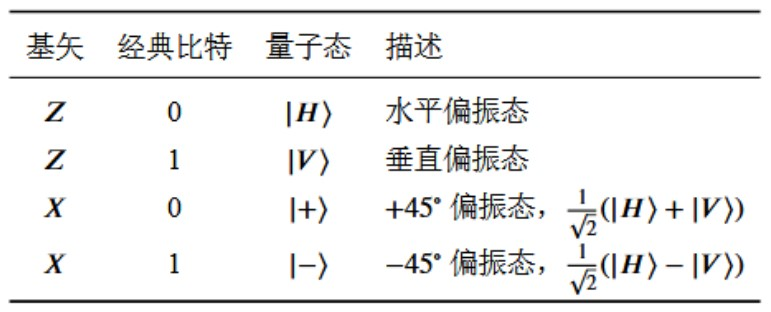
\includegraphics[width=0.9\textwidth]{./fig1.jpg}
        \caption{BB84协议编码表}
    \end{minipage}
\end{figure}

\subsubsection{量子态测量}

作为接收方,Bob 随机从两个基矢$\{Z,X\}$中选择一个对 Alice 发送过来
的单光子态进行测量。若 Bob 选择的基矢和 Alice 制备基矢一致,
则 Bob 测量所得的量子态所对应的经典比特值与 Alice 制备的一致,
否则 Bob 的测量结果将是随机的。重复上述步骤,
直到完成足够的量子态制备和测量后,Alice 和 Bob 各自拥
 有经典比特序列,称之为原始密钥 (Raw Key)。

\subsubsection{基矢比对}

当上述量子信道传输完成后,Bob通过经典信道(经过认证)告知Alice他测
量单光子态时所使用的基矢以及他测量是否得到有效的响应。Alice向Bob公布
她所使用的的基矢。Alice和Bob抛弃掉无测量响应位置的单光子态及制备与测量时使用不同基矢的单光子态,如果制备与测量都是完美的,且没有窃听者Eve对单光子态进行窃听干扰,Alice和Bob此时将得到完全一样的比特值序列。我们称之为筛后密钥(Sifed Key)。

\subsection{经典后处理}

由于信道干扰、制备不完美、测量噪声、窃听者攻击等因素存在,需要对筛后密钥进行经典后处理,才能获得完全相同且安全的最终密钥(Final Key),即安全密钥(Secret Key)。这里经典后处理通常包括误码率估计、比特纠错、隐私放大三个步骤。

\begin{enumerate}
    \item 误码率估计:Alice和Bob经过协商后随机选择筛后密钥的一部分比特进行抽样比对,并计算错误率。若错误率低于设定值,则剩余的密钥继续做后处理,否则中止本次密钥传输。
    \item 比特纠错。为了获得完全相同的密钥,Alice和Bob需要利用纠错算法对剩余的筛后密钥进行纠错,该步骤可以保证在泄露信息尽量小的前提下,Alice和Bob所拥有的密钥产生的错误的概率足够小,即此时Alice和Bob已经拥有完全相同的密钥。
    \item 隐私放大。Alice和Bob通过一定隐私放大算法压缩原始密钥,保证压缩后的密钥被Eve获取信息足够小,最终形成安全密钥(Secret Key)。
\end{enumerate}

\section{实验仪器}

\subsection{量子信号发射器 (Alice)}

量子信号发射机(Alice)机箱主要由发送方主控板、光源板以及Alice光模板组成,主控板控制光源板的四个850nm的激光器随机地发出频率为1MHz的激光脉冲,四路激光发出的光信号是经过调制的,即发出的光是被制备好的四种偏振态,这里记为H、V、+、-;四路光信号通过Alice光模块合成为1路光信号,我们把它称为信号光(Signal),同时主控板的激光器发出一路同步光信号,
波长为1310nm,为信号光提供同步参考。

\subsection{量子信号接收机 (Bob)}

量子信号接收机主要由接收方主控板、单光子探测器(SPD)及接收端光模块组成。主控板根据同步电信号和延时、门宽等参数,让探测器开门探测到接收的光子,单光子探测器SPD是利用雪崩效应探测接收端模块的光子,输出电脉冲信号给主控板处理,主控板根据同步光信号,计算同步光和信号光之间的延时,并根据设定的探测门宽来判别探测到的光子状态。

\subsection{手动偏振控制器 (MPC)}

经过单模光纤传输到接收方的偏振光,由于受到各种因素的影响,例如光纤的椭圆度、残余应力、环境震动以及温度等等,光的偏振态会发生未知的变化,因此接收方用两个MPC,通过调节偏振反馈,来补偿光在路径传输中的偏振变化。

手动偏振控制器是由三个光纤环组成,其功能结构等效为“1/4波片+1/2波片+1/4波片”(第一个环作用是将圆偏振光变成线偏振光,第二个环是将线偏振光补偿旋转一定角度,第三个环的作用是将线偏振光还原为圆偏振光),这样传输到PBS后,相互垂直的偏振光将和PBS的两个轴相吻合,从而被正确的偏振分束。

手动偏振控制器每个环对偏振的调节是按照正弦曲线变化的,因此调节的方法是:先旋转第一个环找到极值点后,接着旋转第二个环找到极值点,然后旋转第三个环,直至偏振达到要求。


\section{实验内容}

以下为实验装置的连接图:

\begin{figure}[H]
    \centering
    \begin{minipage}[b]{0.9\textwidth}
        \centering
        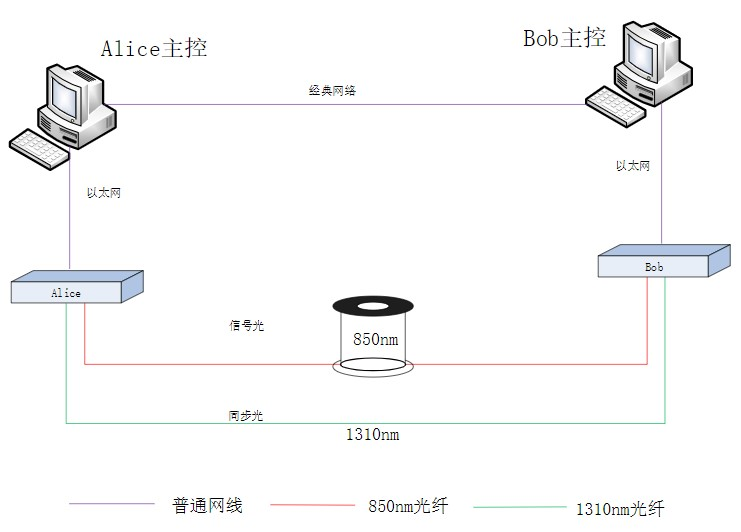
\includegraphics[width=0.9\textwidth]{./fig2.jpg}
        \caption{设备连接图}
    \end{minipage}
\end{figure}

接下来利用软件完成ALice的发送信号,Bob的接受信号以及最后的分析步骤。

\end{document}